\documentclass{article}

\usepackage{graphicx}
\usepackage{subfigure}
\usepackage[hypcap]{caption}
\usepackage{listings}
\usepackage{float}
\floatstyle{plaintop}
\restylefloat{table}

\title{Experimental Design and Data Analysis: Assignment 4}
\author{Andrew Bedard(2566978) \& Simone van Gompel(2567525) \\ Group 19}

\begin{document}

  \maketitle

  \section*{Exercise 1}
    \subsection*{1}
      \begin{lstlisting}[language=R]
      sample_slices = sample(1:18, 18)
      \end{lstlisting}
    
    \subsection*{2}
      \begin{figure}[H]
          \centering
          \subfigure[Humidity]
          {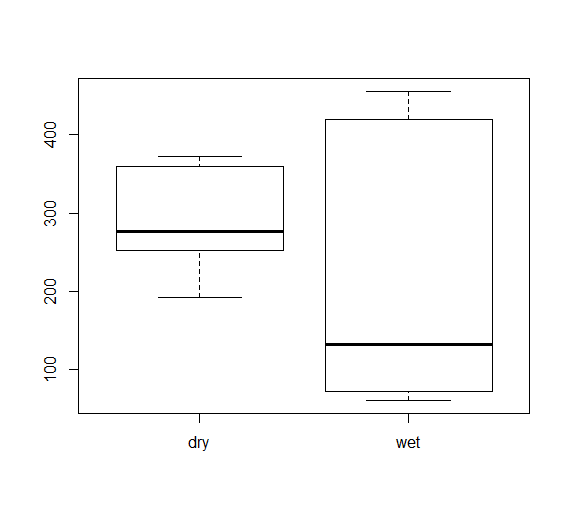
\includegraphics[scale=0.2]{../results/BoxHoursHum.png} }
          \subfigure[Environment]
          {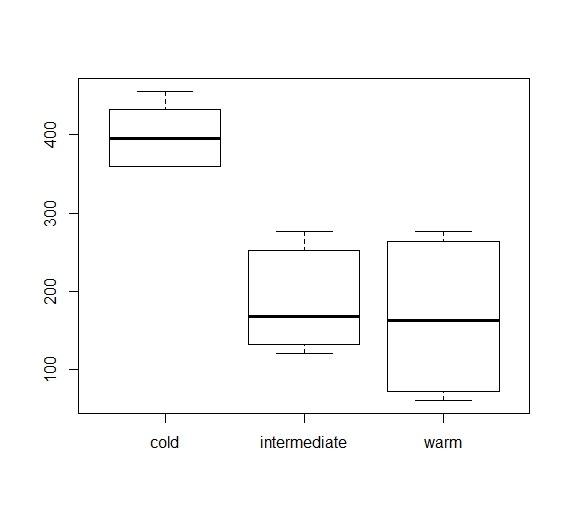
\includegraphics[scale=0.2]{../results/BoxHoursEnv.png} }
          \caption{Boxplots of Hours with Humidity and Environment}
          \label{fig:BoxHours}
      \end{figure} 
    
    \subsection*{3}
      \begin{figure}[H]
          \centering
          \subfigure[Humidity]
          {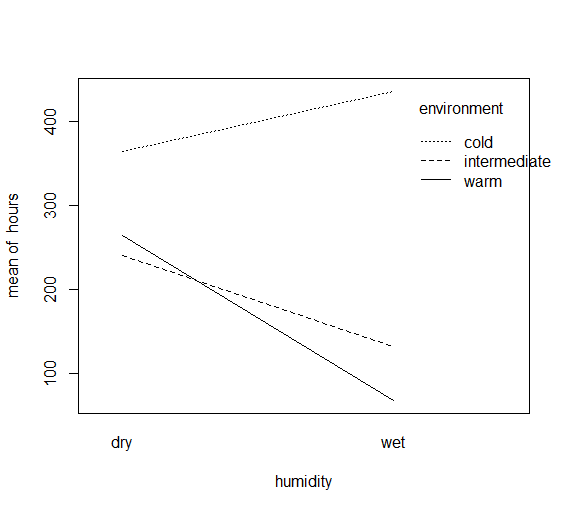
\includegraphics[scale=0.2]{../results/IntPlotHoursHum.png} }
          \subfigure[Environment]
          {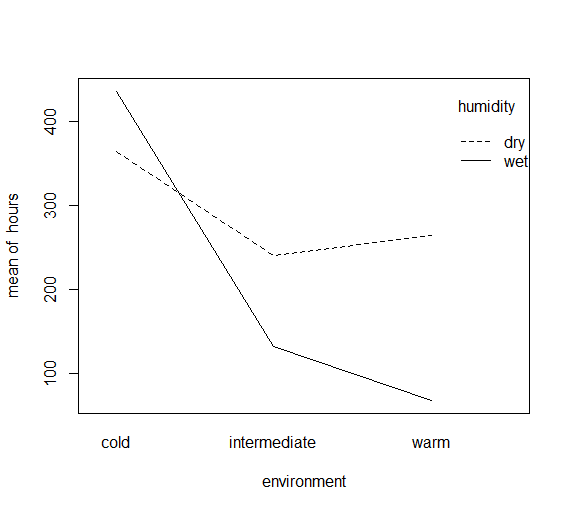
\includegraphics[scale=0.2]{../results/IntPlotHoursEnv.png} }
          \caption{Interactionplots of Hours with Humidity and Environment}
          \label{fig:IntPlotHours}
      \end{figure}
    
    \subsection*{4}
      Analysis of variance on both factors:\\\\
      \begin{lstlisting}[language=R]
Analysis of Variance Table

Response: hours
            Df Sum Sq Mean Sq F value    Pr(>F)    
environment  2 201904  100952 23.1057 3.674e-05 ***
humidity     1  26912   26912  6.1596   0.02637 *  
Residuals   14  61168    4369                      
---
Signif. codes:  0 ‘***’ 0.001 ‘**’ 0.01 ‘*’ 0.05 ‘.’ 0.1 ‘ ’ 1
      \end{lstlisting}
    
    \subsection*{5}
    
    \subsection*{6}
    
    \subsection*{7}
    
    \subsection*{8}
    
  \section*{Exercise 2}
    \subsection*{1}
     
    \subsection*{2}
	\begin{figure}[H]
		\centering
          \subfigure[]
          {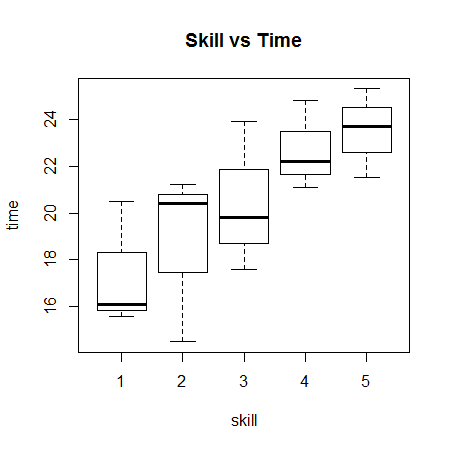
\includegraphics[scale=0.35]{../results/2_2_1.png} }
          \subfigure[]
          {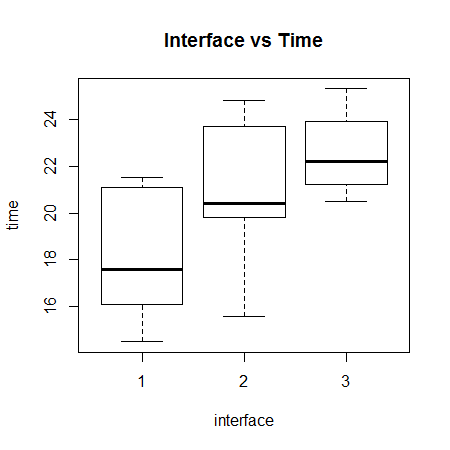
\includegraphics[scale=0.35]{../results/2_2_2.png} }
          \caption{Box Plots of Skill and Interface vs Time}
          \label{fig:srchbox}
	\end{figure}
	
	\begin{figure}[H]
	\centering
		\subfigure[]
          {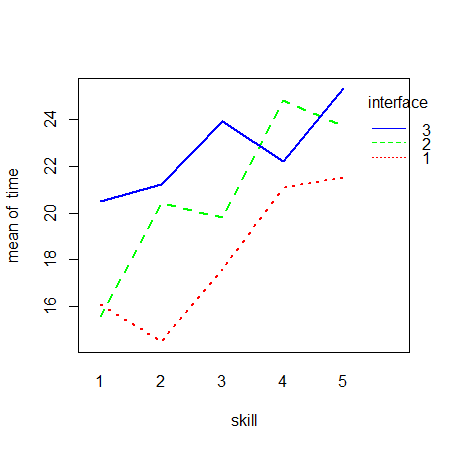
\includegraphics[scale=0.35]{../results/2_2_3.png} }
          \subfigure[]
          {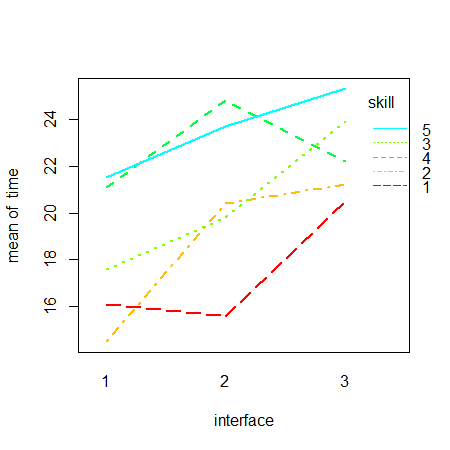
\includegraphics[scale=0.35]{../results/2_2_4.png} }
          \caption{Interaction plots of Skill and Interface vs Time}
          \label{fig:srch_interaction}
	\end{figure}
	
	It is difficult to conclude that there is an interaction between skill and interface as they are clearly not parallel, but they follow the same general trajectory, so this interaction may be due to noise. 
    \subsection*{3}
    Using the Kurskal-Wallis rank sum test, we test if the distributions of our populations in regards to the time measured for different interfaces are the same, and we obtain the following results:\\\\
      \begin{lstlisting}[language=R]
Kruskal-Wallis rank sum test

data: time and interface
Kruskal-Wallis chi-squared = 4.22, df = 2, p-value =0.1212
      \end{lstlisting}
      Thus with a p-value of 0.1212 we reject the null hypothesis that our populations are the same, therefore the search time for all interfaces is not equal.
    \subsection*{4}
    
    \subsection*{5}
    \begin{figure}[H]
    \centering
    	\subfigure[]
		{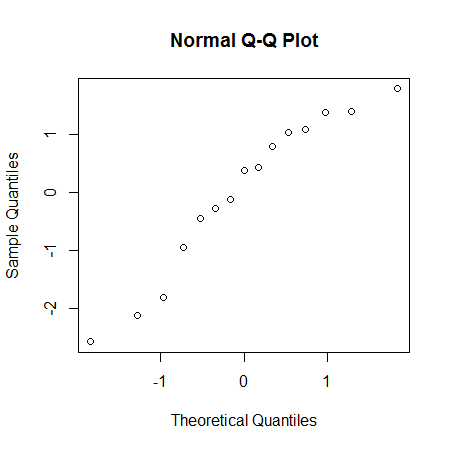
\includegraphics[scale=0.35]{../results/2_5_1.png} }
        \subfigure[]
        {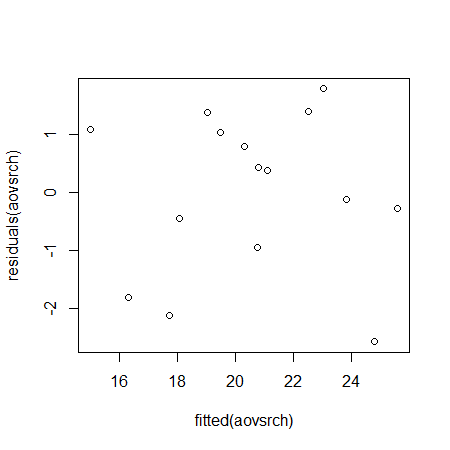
\includegraphics[scale=0.35]{../results/2_5_2.png} }
        \caption{Diagnostic Plots}
        \label{fig:diagnostic}
    \end{figure}
    It is difficult to say for certain, there may be a slight curve in the qq-plot \ref{fig:diagnostic}(a) but it looks approximately normal, and the fitted value plot \ref{fig:diagnostic}(b) suggests there is no significant difference in the population variances.
    \subsection*{6}
	\begin{lstlisting}[language=R]
Friedman rank sum test

data: time, interface and skill
Friedman chi-squared = 6.4, df = 2, p-value = 0.04076
	\end{lstlisting}
	With a p-value of 0.04076 we reject the null hypothesis, thus we conclude there is an effect of interfaces.
    \subsection*{7}
    Testing the null hypothesis that the search time is the same for all interface by a ANOVA test, ignoring skill we obtain the following:
    \begin{lstlisting}[language=R]
    Analysis of Variance Table

Response: time
          Df  Sum Sq Mean Sq F value  Pr(>F)  
interface  2  50.465  25.233  2.8605 0.09642 .
Residuals 12 105.852   8.821                  
---
Signif. codes:  
0 ‘***’ 0.001 ‘**’ 0.01 ‘*’ 0.05 ‘.’ 0.1 ‘ ’ 1
	\end{lstlisting}
	With a p-value of 0.09642 we do not reject the null hypothesis, thus the time is not the same for all interfaces.
	This test is useful to use, if some conditions are met, as of right now, we do not have convincing evidence there is no interaction between skill and interface. It would be more useful to test along with the variable skill, and the interaction between the two as follows:
	    \begin{lstlisting}[language=R]
	Analysis of Variance Table

Response: time
                Df Sum Sq Mean Sq F value    Pr(>F)    
interface        1 49.729  49.729 21.4145 0.0007313 ***
skill            1 78.732  78.732 33.9039 0.0001154 ***
interface:skill  1  2.312   2.312  0.9956 0.3398204    
Residuals       11 25.544   2.322                      
---
Signif. codes:  
0 ‘***’ 0.001 ‘**’ 0.01 ‘*’ 0.05 ‘.’ 0.1 ‘ ’ 1
	\end{lstlisting}
	This way we are able to measure the interaction between the data sets, and determine whether there is a factor which has a greater effect on our results. From the previous table we see that with a p-value of 0.3398 we accept the null hypothesis that there is no significant interaction between skill in and interface, which is what we require for the one-way ANOVA ignoring skill to be valid.
  \section*{Exercise 3}
    \subsection*{1}
      \begin{lstlisting}[language=R]
Analysis of Variance Table

Response: acidity
          Df Sum Sq Mean Sq F value   Pr(>F)   
starter    4 44.136 11.0340  8.0835 0.001106 **
batch      1  4.855  4.8547  3.5566 0.078826 . 
position   4  2.348  0.5870  0.4300 0.784786   
Residuals 15 20.475  1.3650                    
---
Signif. codes:  0 ‘***’ 0.001 ‘**’ 0.01 ‘*’ 0.05 ‘.’ 0.1 ‘ ’ 1
      \end{lstlisting}
      
    
    \subsection*{2}
      \begin{lstlisting}[language=R]
Call:
lm(formula = acidity ~ starter + batch + position, data = cream)

Residuals:
    Min      1Q  Median      3Q     Max 
-1.7512 -0.7596  0.0132  0.8816  1.0856 

Coefficients:
            Estimate Std. Error t value Pr(>|t|)    
(Intercept)   7.8260     0.8586   9.115 1.67e-07 ***
starter2     -0.1500     0.7389  -0.203  0.84186    
starter3     -0.9800     0.7389  -1.326  0.20459    
starter4      2.8100     0.7389   3.803  0.00173 ** 
starter5     -0.4840     0.7389  -0.655  0.52238    
batch         0.3116     0.1652   1.886  0.07883 .  
position2    -0.6180     0.7389  -0.836  0.41608    
position3    -0.0380     0.7389  -0.051  0.95966    
position4    -0.7640     0.7389  -1.034  0.31755    
position5    -0.2640     0.7389  -0.357  0.72586    
---
Signif. codes:  0 ‘***’ 0.001 ‘**’ 0.01 ‘*’ 0.05 ‘.’ 0.1 ‘ ’ 1

Residual standard error: 1.168 on 15 degrees of freedom
Multiple R-squared:  0.7149,  Adjusted R-squared:  0.5438 
F-statistic: 4.179 on 9 and 15 DF,  p-value: 0.007304
      \end{lstlisting}
      \label{tble:estimates}

    \subsection*{3}
      \begin{lstlisting}[language=R]
Linear Hypotheses:
           Estimate Std. Error t value Pr(>|t|)    
2 - 1 == 0  -0.1500     0.4673  -0.321    0.997    
3 - 1 == 0  -0.9800     0.4673  -2.097    0.282    
4 - 1 == 0   2.8100     0.4673   6.013   <0.001 ***
5 - 1 == 0  -0.4840     0.4673  -1.036    0.834    
3 - 2 == 0  -0.8300     0.4673  -1.776    0.429    
4 - 2 == 0   2.9600     0.4673   6.334   <0.001 ***
5 - 2 == 0  -0.3340     0.4673  -0.715    0.949    
4 - 3 == 0   3.7900     0.4673   8.110   <0.001 ***
5 - 3 == 0   0.4960     0.4673   1.061    0.822    
5 - 4 == 0  -3.2940     0.4673  -7.048   <0.001 ***
      \end{lstlisting}
      \label{tble:p-values}
        Starter 1 and 4 produce significantly different acidity. This is apparent first from exercise 3.2 we obtain: $\mu_1 = 7.8260$ and $\mu_4 = 7.8260 + 2.8100 = 10.636$ which are the estimates for starter 1 and 4 respectively. Furthermore the p-value for starter 1 obtained from exercise 3.2, of 1.67e-07 suggests that we reject the null hypothesis that our estimate for starter 1 is equal to that of the rest of the population, and the p-values obtained from the simultaneous method, of 0.001 suggests that we reject the null hypothesis that the estimate for the treatment effect of 4 is equal to each of the other respective treatment effects.
    \subsection*{4}
    The p-value for the test $H_0: \alpha_2 = \alpha_1$, where $\alpha_i$ is our estimate of the treatment effects is 0.997, whereas in exercise 3.2 our p-value for the null hypothesis $H_0: \alpha_2 = \alpha_1$ is 0.84186. It is no coincidence that the p-value obtained from exercise 3.2, is different from that of the simultaneous calculation, this is due to the fact that when calculating the simultaneous p-values for the null hypothesis  $H_0: \alpha_i = \alpha_1$ we are doing so in such a way that the probability of rejecting any null hypothesis in error is less than 0.5. In contrast to the method used in exercise 3.2, where for every null hypothesis our chance of making such an error is $N*0.05$ where N is the number of possibilities to make such an error. In this way the Simultaneous p-values method gives us a higher confidence in our conclusions.
    \subsection*{5}
      \begin{lstlisting}[language=R]
Linear Hypotheses:
           Estimate lwr     upr    
2 - 1 == 0 -0.1500  -1.6391  1.3391
3 - 1 == 0 -0.9800  -2.4691  0.5091
4 - 1 == 0  2.8100   1.3209  4.2991
5 - 1 == 0 -0.4840  -1.9731  1.0051
3 - 2 == 0 -0.8300  -2.3191  0.6591
4 - 2 == 0  2.9600   1.4709  4.4491
5 - 2 == 0 -0.3340  -1.8231  1.1551
4 - 3 == 0  3.7900   2.3009  5.2791
5 - 3 == 0  0.4960  -0.9931  1.9851
5 - 4 == 0 -3.2940  -4.7831 -1.8049
      \end{lstlisting}
    The confidence intervals for testing all differences $\alpha_j - \alpha_{j'}$ for $(i,i' \in {1,2...,5})$ of the main effects for starter with simultaneous confidence level 95\% are (4-1),(4-2),(4-3),(4-5),(5-4) so all those containing starter 4. This is likely due to the fact that the estimated value for starter 4, which was earlier calculated as 10.636, is so much larger than every other estimate, for example all the confidence intervals for (4-i) are greater than 0, and the one interval (5-4) is less than 0.
  \section*{Exercise 4}
    \subsection*{1}
    
    \subsection*{2}
    
    \subsection*{3}
    
    \subsection*{4}

    
  \section{R-Code}
    \subsection{Exercise 1}\label{sec:RE1}
      \begin{lstlisting}[language=R]
      \end{lstlisting}
    \subsection{Exercise 2}\label{sec:RE2}
      \begin{lstlisting}[language=R]
      \end{lstlisting}
    \subsection{Exercise 3}\label{sec:RE3}
      \begin{lstlisting}[language=R]
      \end{lstlisting}
    \subsection{Exercise 4}\label{sec:RE4}
      \begin{lstlisting}[language=R]
      \end{lstlisting}
\end{document}
